\documentclass[9pt]{acm_proc_article-sp}
\usepackage{graphicx}
\usepackage{amsmath}
\usepackage{enumerate}
\usepackage{multirow}
\usepackage{epstopdf}
\usepackage{array}
\usepackage{CJK}
\usepackage{float}
\usepackage{subfigure}
\usepackage{algorithm}
\usepackage{algorithmicx}
\newcommand{\algorithmicbreak}{\textbf{break}}
\newcommand{\BREAK}{\State \algorithmicbreak}
\usepackage{algpseudocode}
\begin{document}

\title{AVERec: A random walk based academic venue recommendation model}

\numberofauthors{1}
\author{
% 1st. author
\alignauthor
Zhen Chen, Huizhen Jiang, Haifeng Liu\\
       \affaddr{School of Software, Dalian University of Technology, Dalian 116620, China.}\\
       \email{f.xia@acm.org}
%% 2nd. author
%\alignauthor
%G.K.M. Tobin\titlenote{The secretary disavows
%any knowledge of this author's actions.}\\
%       \affaddr{Institute for Clarity in Documentation}\\
%       \affaddr{P.O. Box 1212}\\
%       \affaddr{Dublin, Ohio 43017-6221}\\
%       \email{webmaster@marysville-ohio.com}
%% 3rd. author
%\alignauthor Lars Th{\o}rv{\"a}ld\titlenote{This author is the
%one who did all the really hard work.}\\
%       \affaddr{The Th{\o}rv{\"a}ld Group}\\
%       \affaddr{1 Th{\o}rv{\"a}ld Circle}\\
%       \affaddr{Hekla, Iceland}\\
%       \email{larst@affiliation.org}
%\and  % use '\and' if you need 'another row' of author names
%% 4th. author
%\alignauthor Lawrence P. Leipuner\\
%       \affaddr{Brookhaven Laboratories}\\
%       \affaddr{Brookhaven National Lab}\\
%       \affaddr{P.O. Box 5000}\\
%       \email{lleipuner@researchlabs.org}
%% 5th. author
%\alignauthor Sean Fogarty\\
%       \affaddr{NASA Ames Research Center}\\
%       \affaddr{Moffett Field}\\
%       \affaddr{California 94035}\\
%       \email{fogartys@amesres.org}
%% 6th. author
%\alignauthor Charles Palmer\\
%       \affaddr{Palmer Research Laboratories}\\
%       \affaddr{8600 Datapoint Drive}\\
%       \affaddr{San Antonio, Texas 78229}\\
%       \email{cpalmer@prl.com}
}
% There's nothing stopping you putting the seventh, eighth, etc.
% author on the opening page (as the 'third row') but we ask,
% for aesthetic reasons that you place these 'additional authors'
% in the \additional authors block, viz.
%\additionalauthors{Additional authors: John Smith (The Th{\o}rv{\"a}ld Group,
%email: {\texttt{jsmith@affiliation.org}}) and Julius P.~Kumquat
%(The Kumquat Consortium, email: {\texttt{jpkumquat@consortium.net}}).}
%\date{30 July 1999}
% Just remember to make sure that the TOTAL number of authors
% is the number that will appear on the first page PLUS the
% number that will appear in the \additionalauthors section.

\maketitle
\begin{abstract}
In this work, we propose AVERec, a novel random walk based academic venue recommendation model. AVERec models the co-publishing network with two kinds of associations, i.e. co-author relations and author-venue relations. We exploit three academic factors to define a transfer matrix with bias which drives a random walk with restart model running on the co-publishing network. The three academic factors, i.e. co-publishing frequency, weight of relations and similar-level preferred, are inspired by that, researchers are more likely to contact academic entities with high co-publishing frequency and similar academic level, as well as the weight of the two kinds of associations should be differentiated. We conduct extensive experiments on DBLP data set in order to measure AVERec. The results demonstrate that AVERec significantly improves the performance on precision, recall and F1 when compared to the baseline method.
\end{abstract}

% A category with the (minimum) three required fields
\category{H.4}{Information Systems Applications}{Miscellaneous}
%A category including the fourth, optional field follows...
\category{D.2.8}{Software Engineering}{Metrics}[complexity measures, performance measures]

\terms{Theory}

\keywords{ACM proceedings, \LaTeX, text tagging}

\section{Introduction}
Introduction...
\section{Related work}
Related work...
\section{Academic Venue Recommendation Model}
The AVERec academic venue recommendation model is designed to mine specific academic venues and make personalized recommendation for researchers. The model is inspired by the truth that, researchers usually desire to contact with suitable academic venues, i.e. keep concern on high-quality and fruitful academic venues, participate in academic conferences which are closely related to their research, contribute to some venues in where they are possible to publish research achievements. Besides, AVERec is a evolution from a basic RWR model which has been proved to be competent for calculating the similarity of nodes in networks. Most of all, the three academic factors we introduced, co-publishing frequency, weight of relations and similar-level preferred, aim at biasing the random walk, such that it will more easily traverse to the positive nodes. The detailed process of AVERec is described below. Additionally, the structure is illustrated in Figure~\ref{Fig1}.
\begin{figure}[!ht]
\centering
\includegraphics [width=3.5in]{Fig1.pdf}
\caption{The structure of AVERec.}
\label{Fig1}
\end{figure}
\subsection{Overview of AVERec}
In this work, we model a kind of co-publishing networks which are characterized by researchers and academic venues. Figure~\ref{Fig2} shows an example of the network. The colorized nodes represent venues A, B, C and D. As well as the three researchers Bob, David and Alice collaborate to write five papers which are published in the four venues respectively (note that Bob publish two papers in venue A). The nodes (venues and researchers) along with links (co-author relations and author-venue relations) form the co-publishing networks. We define two kinds of node sets, $Venues$ and $Authors$.
\begin{figure}[!ht]
\centering
\includegraphics [width=2.5in]{Fig2.pdf}
\caption{An example of co-publishing network.}
\label{Fig2}
\end{figure}
In AVERec academic venue recommendation model, whether a venue should be recommended depends on its importance to the target researcher. The importance is defined by the rank score of the venue, which is determined by two factors, i.e. the number of neighbor nodes and the rank score of incident nodes. Equation~\ref{equ1} describes this theory.
\begin{equation}
\label{equ1}
AR(p_{i})=\frac{1-\alpha}{N}+\alpha \sum_{p_{j}\in A(p_{i})}AR(p_{j})P(p_{j},p_{i})
\end{equation}
$AR$ represents the rank score vector. $AR(p_{i})$ is the rank score of node $p_{i}$. $A(p_{i})$ is the set of nodes incident to node $p_{i}$. $P(p_{j},p_{i})$ is the transition probability from node $p_{j}$ to node $p_{i}$. $\alpha$ is the damping factor. When the AVERec is run on the network to compute node ranking. Starting from source node $p_{0}$, an imaginary walker randomly walk in the network. The walker has two choice, i.e. with probability $\alpha$, walk to next node $p_{x}$, which is one of $p_{0}$'s direct neighbors ($p_{x}\in A(p_{0})$), with probability $1-\alpha$, return to source vertex $p_{0}$. Equation~\ref{equ1} represents one step to get rank score for node $p_{i}$. With respect to all node in the whole network, the approach is defined by equation~\ref{equ2}, which is an iterative process.
\begin{equation}
\label{equ2}
AR^{(t+1)}=\alpha \mathbf{S}AR^{(t)}+(1-\alpha)q
\end{equation}
$AR^{t}$ is the rank score vector at step $t$. $q$ is a row vector $(0,...,1,...,0)$. It should be noticed that, $AR_{0}=q$. The rank score of target node is $1$, while others' are $0$. $\mathbf{S}$ is the transfer matrix, representing the probability for each node to skip to next node. For basic RWR model, the cell of matrix $\mathbf{S}$ (i.e. $P(p_{j},p_{i})$ in Equation~\ref{equ1}) is defined as $\frac{1}{L(p_{i})}$. ($L(p_{i})$ is the number of node $p_{i}$'s neighbors). It means that, the walker have same probability to skip to next node. In AVERec, we do some guidance work by introducing three academic factors. The change of $P(p_{j},p_{i})$ can lead the walker skips with preference, which will be proved to be better in section~\ref{section:evaluation} for academic venue recommendation.

The detailed process of AVERec is described below corresponding with the structure in Figure~\ref{Fig1}.

\begin{itemize}
  \item \emph{Step1}. The initial input data is a set of publications with authors' information and venues' information. AVERec firstly extracts the co-author relations and author-venue relations. Then, generates the co-publishing networks. There is a link between two authors if they coauthored at least one paper, as well as a link between researcher and venue if the researcher published a paper in the venue.
  \item \emph{Step2}. Following initializing the rank score of nodes and weight of edges, AVERec run on the network. During the random walk process, the walker skip to next node with a modified probability by considering the three academic factors. The walk will stop until the rank score is approximately convergent or the iterations come to upper limit.
  \item \emph{Step3}. After getting the convergent rank score of each node, AVERec sorts the venue in accordance to their corresponding rank scores. Finally, removing the venues with which the target author have contacted, the Top-N venues are recommended to the target author.
\end{itemize}

We present below the details of how the transfer matrix with bias is computed by considering the three academic factors.

\subsection{Transfer Matrix with Bias}
As the example shown in Figure~\ref{Fig2}, there are seven academic entities. With respect to recommending venues to Bob, he has never contacted with venue C and D. According to the characteristics of the random walk with restart model, the walker can walk from Bob to C and D via David and Alice respectively. After several times iterative walking, venues C and D are recommended to Bob based on the sorted rank score. However, there are several academic factors that can be introduced to meet the real scene. We exploit three of them to redefine the transfer matrix in random walk with restart model.

Generally, researchers prefer contact the academic entities (researchers and venues) which have high frequency of interaction with them, i.e. high publishing frequency in the venue or high collaborating frequency with the researchers. As shown in Figure~\ref{Fig2}, we think Bob prefer contacting David rather than Alice, because Bob collaborated with David twice while Alice once. David looks more important than Alice for Bob. As well as Bob prefer contacting venue A rather than B, since that Bob published two papers in venue A. Based on this assumption, We define co-publishing frequency as Equation~\ref{equ3} which is a part of the links' weight.
\begin{equation}
\label{equ3}
F_{i,j}=\left\{\begin{array}{ll}
cp_{i,j} & i\in Author,\quad j\in Venues\\
ct_{i,j} & i,j\in Authors\\
\end{array}\right.
\end{equation}
Where $cp_{i,j}$ is the count of author $i$'s publications in venue $j$. $ct_{i,j}$ is $i$'s collaborating times with author $j$.

In addition, there are two kinds of associations in co-publishing networks, i.e. co-author relations and author venue relations. In case of basic random walk model, the difference between these two relations is ignored. Author-venue relations seems more important than co-author relations, because the event of publishing a paper in the venue is more ponderable when profiling the researchers' interest. This proposition has been proved in subsequent experiment which can lead better performance when making academic recommendation. We measure the weight of relations by Equation~\ref{equ4} based on a ratio $\beta$.
\begin{equation}
\label{equ4}
W_{i,j}=\beta F_{i,j}
\end{equation}
The ratio $\beta$ is a variable empirical value. In our experiments, $\beta$ is set as 20 for author-venue relations and 1 for co-author relations.

Finally, we proposed an assumption: the interest features of academic entities can be more accurately reflected by similar level neighbors. In case of researchers, they prefer contacting other researchers at similar academic levels and publishing papers in the venue which have potential to accept. In other words, the relations between similar-level academic entities are more weighty. The walker should walk along these nodes with more probability in AVERec. In order to measure the similarity of academic entities, we define a simple metric as equation~\ref{equ5}.
\begin{equation}
\label{equ5}
LevSim_{i,j}=1-\frac{\Vert AR_{i}-AR_{j}\Vert}{\max_{x\in L(i)}(\Vert AR_{i}-AR_{x}\Vert)}
\end{equation}
This Equation~\ref{equ5} aim at finding the neighbor with smallest rank score disparities based on a normalization method. When computing the transfer probability $S_{i,j}$ from node $i$ to node $j$, our AVRec model adopts equation~\ref{equ6}. With equation~\ref{equ6}, the walker can run on the network with modified bias.
\begin{equation}
\label{equ6}
\mathbf{S}_{i,j}=\frac{W_{i,j}}{\sum_{x\in L(i)}W_{i,x}}LevSim_{i,j}
\end{equation}

\section{Evaluation and analysis}
\label{section:evaluation}
We conducted extensive experiments using data from DBLP~\cite{Ley:DBLP}, a computer science bibliography website hosted at University Trier. In this section, we describe three academic venue recommendation approaches as comparison, the statistics of data set, the evaluation metrics and our experimental procedure for evaluating the performance of AVRec, as well as detailed analysis of the results.

\subsection{Three Comparison Approaches}
To measure the performance of AVERec, we conducted three comparison approaches, i.e. the basic random walk with restart model (RWR), a topic-based model and a friends-based model.

Similar to popular random walk models, the details and verification method of RWR is just like AVERec, except for the definition of transfer matrix with bias. The topic-based method is a content-based recommendation approach in the strict sense. The core of the approach is to compute the similarity between researchers and venues. In this implementation, we regarded the topic distribution of researchers' publications content and venues's publications content as feature vector respectively, which is calculated by LDA(Latent Dirichlet Allocation) model~\cite{blei2003latent}. The similarity of researchers and venues is defined by the Cosine Similarity based on these feature vectors. The friends-based model is a kind of collaborative filtering recommendation approach. Its basis of recommending venues is the number of neighbors who have relations with the venues. In this implementation, we treat researcher's collaborators and "collaborators of collaborator" as neighbors. If there are many neighbors contact a venue, the venue should be recommended to the researcher.

\subsection{Data Set and Metrics}
DBLP indexes more than 2.3 million articles on computer science. In our experiments, we use a subset of DBLP. The subset data are all in the field of data mining involving 34 journals and 38 conferences altogether. The statistics about the data sets are shown in Table~\ref{table1}. The data set contain 74 venues and 70326 researches. 163446 articles connect researchers and venues, as well as come into being the co-publishing networks. We divided the data set into two parts: the data before year 2011 as a training set, and others as a testing set.

\begin{table}
\renewcommand{\arraystretch}{1.2}
\centering
\caption{Statistics of Data Set from DBLP}
\label{table1}
\begin{tabular}{|c|c|c|c|} \hline
Statistics &venues&researchers&articles\\ \hline
Number & 74 & 70326 &163446 \\
\hline\end{tabular}
\end{table}

The detailed statistical characteristic of this co-publishing network is shown in Figure~\ref{fig3}. Figure~\ref{fig3}(a) describes the scale of participants or contributors for each venue. Almost half of the venues keep no more than 500 researchers. The scales of 11 venues are so large that up to 3000 researchers publish papers on them. We can also get that from Figure~\ref{fig3}(b), almost $94$ percentage of these 70326 researchers contact no more than 3 venues. However, there are also some "academic stars" contribute more than 14 venues, which account for $0.13\%$. Similarly, Figure~\ref{fig3}(c) shows the same trend for number of researchers' publications. Most of them published no more than five papers, but there are also many researchers published more than 14 papers. Figure~\ref{fig3}(d) shows the number of co-authors for each researchers. We can conclude that, the degrees of most researchers are under 14, which indicate that this data set is very sparse.

\begin{figure}[!ht]
\centering
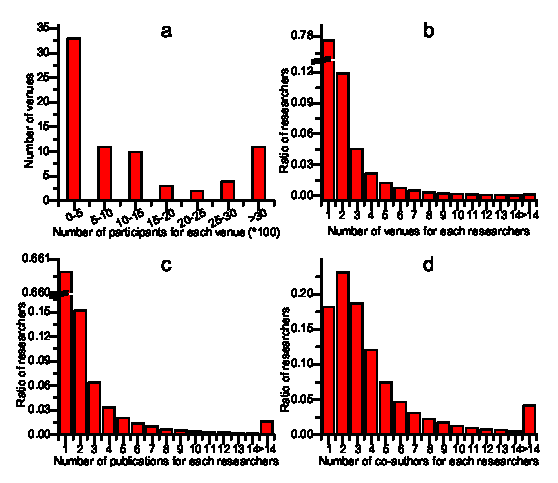
\includegraphics [width=3.5in]{Fig3.eps}
\caption{Detailed statistics of the data set from DBLP}
\label{fig3}
\end{figure}

We use three popular metrics, precision, recall and F1 score, to evaluated the performance of AVERec. Detailed information about these metrics have been discussed in~\cite{xia2014mvcwalker}. All experiments were performed on a 64-bit Linux-based operation system, Ubuntu 12.04 with a 4-duo and 3.2-Ghz Intel CPU, 8-G Bytes memory. All the programs are implemented with Python.

\subsection{Results and Analysis}
In this section, we firstly conducted several experiments about AVERec, basic RWR, topic-based and friends-based recommendation model on aforesaid data set. Secondly, we measured the performance of AVERec when recommending academic venues for researchers at different levels. We randomly chose 100 researchers as target nodes. Additionally, AVERec and RWR model are run with the damping factor 0.8.

\begin{figure*}[t]
\centering
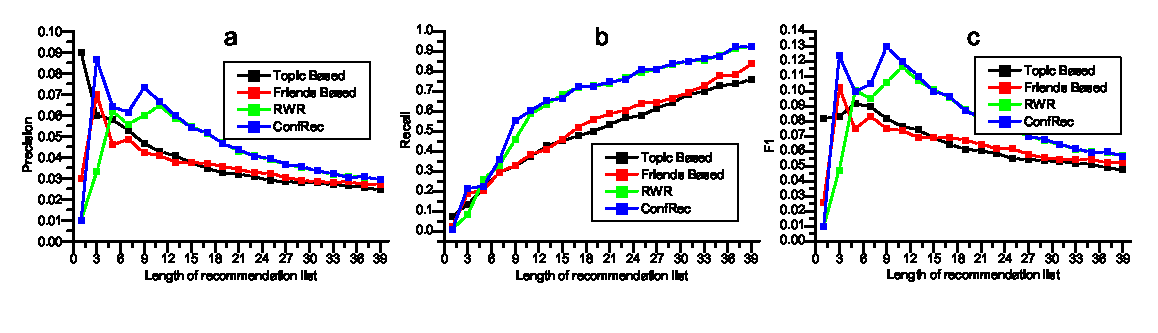
\includegraphics [width=\textwidth]{Fig4.eps}
\caption{Performance of AVERec, basic RWR, topic-based and friends-based recommendation model}
\label{fig4}
\end{figure*}

\begin{figure*}[t]
\centering
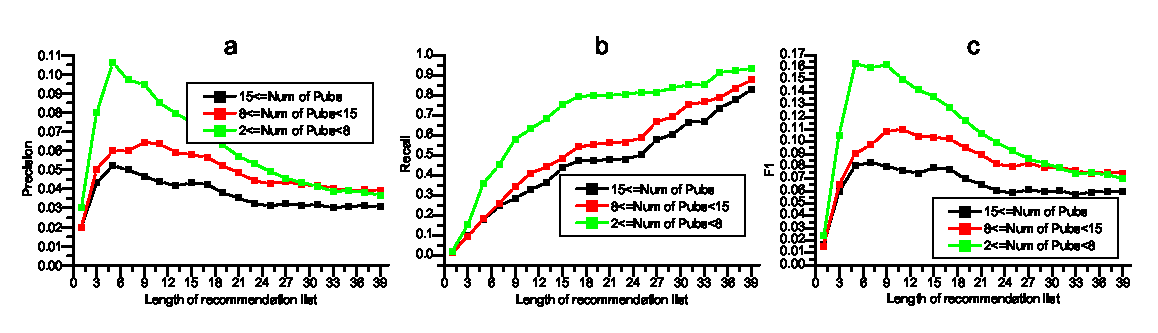
\includegraphics [width=\textwidth]{Fig5.eps}
\caption{The impact of researchers' publications number on AVERec.}
\label{fig5}
\end{figure*}

Figure~\ref{fig4} shows the performance of AVERec, basic RWR, topic-based and friends-based recommendation model. The $x$ axis represents the length of recommendation list, which is range in 1 to 39. the $y$ axis represents precision, recall and F1 score respectively. In case of Figure~\ref{fig4}(a), all lines roughly show coincident downtrend. However, AVERec and basic RWR performs better in precision as a whole. On the view of range 1 to 11 on $x$ axis, AVRec get higher precision, as well as that it come to a peak value $8.7\%$ at point 3. With the growth of recommendation list, the performance of the four recommendation approach tend to be similar.In case of Figure~\ref{fig4}(b), the lines rise obviously. AVERec and basic RWR have no significant difference, but the their recall performs better than that of topic-based and friend-based approach. With the number of recommended venues level off to the sum of venues, the recall approach 1. According to Figure~\ref{fig4}(c), the F1 score shows similar trend with precision. The F1 score of AVERec reaches the highest value of $12.95\%$ when recommend 9 venues for each researchers. The upgrade rate is $11.3\%$ comparing to basic RWR. It is worth mentioning that, AVERec reaches its peak at point 9, while basic RWR get highest F1 score at point 11. That means the recommendation efficiency of AVERec is higher.

These experiments demonstrated that, the random walk with restart based model can get more accurate academic venue recommendation than topic based and friend based approaches. What's more, our work on transfer matrix with bias do improve the performance of AVERec, and make it more efficient.

We also made several extensive experiments to measure the performance of AVERec on different researchers. We mainly focused on the difference of researchers academic level, which is reflected by the number of publications. Generally, the newcomer shows lower academic level with few publications, while a fruitful professor show high academic level with a mount of high-quality publications. We divided the researchers into three sets, i.e. $C1$ contains researchers whose publications number range from 2 to 8,$C2$ contains researchers with 8 to 15 publications and $C3$ contains researchers with more than 15 publications. The experimental results are show in Figure~\ref{fig5}.


From Figure~\ref{fig5}, we can see significant difference of the effect on different sets of researchers even though they show a similar trend in precision, recall and F1 score respectively. In Figure~\ref{fig5}(c), Especially the AVERec can get highest value $16.24\%$ of F1 score at point 9 when making academic venues recommendation for the researchers with 2 to 8 publications. The results mean that, AVERec can do better at recommending academic venues for researchers with fewer publications, i.e. the relatively newcomer, which meet our original intention of recommending academic venues for newcomer well.
%\begin{table}
%\centering
%\caption{Frequency of Special Characters}
%\begin{tabular}{|c|c|l|} \hline
%Non-English or Math&Frequency&Comments\\ \hline
%\O & 1 in 1,000& For Swedish names\\ \hline
%$\pi$ & 1 in 5& Common in math\\ \hline
%\$ & 4 in 5 & Used in business\\ \hline
%$\Psi^2_1$ & 1 in 40,000& Unexplained usage\\
%\hline\end{tabular}
%\end{table}


%\begin{table*}
%\centering
%\caption{Some Typical Commands}
%\begin{tabular}{|c|c|l|} \hline
%Command&A Number&Comments\\ \hline
%\texttt{{\char'134}alignauthor} & 100& Author alignment\\ \hline
%\texttt{{\char'134}numberofauthors}& 200& Author enumeration\\ \hline
%\texttt{{\char'134}table}& 300 & For tables\\ \hline
%\texttt{{\char'134}table*}& 400& For wider tables\\ \hline\end{tabular}
%\end{table*}
% end the environment with {table*}, NOTE not {table}!


%
%\begin{figure}
%\centering
%\epsfig{file=fly.eps, height=1in, width=1in}
%\caption{A sample black and white graphic (.eps format)
%that has been resized with the \texttt{epsfig} command.}
%\end{figure}

%
%\begin{figure}
%\centering
%\psfig{file=rosette.ps, height=1in, width=1in,}
%\caption{A sample black and white graphic (.ps format) that has
%been resized with the \texttt{psfig} command.}
%\end{figure}

%\begin{figure*}
%\centering
%\epsfig{file=flies.eps}
%\caption{A sample black and white graphic (.eps format)
%that needs to span two columns of text.}
%\end{figure*}
\section{Conclusions}

%\end{document}  % This is where a 'short' article might terminate

%ACKNOWLEDGMENTS are optional
\section{Acknowledgments}

\bibliographystyle{abbrv}
\bibliography{ConfRec}
\appendix
%Appendix A
\balancecolumns
\end{document}
